%%%%%%%%%%%%%%%%%%%%%%%%%%%%%%%%%%%%%%%%%%%%%%%%%%%%%%%%%%%%%%%%%%%%%%%%%%%%%%%%%%%%
% Document data
%%%%%%%%%%%%%%%%%%%%%%%%%%%%%%%%%%%%%%%%%%%%%%%%%%%%%%%%%%%%%%%%%%%%%%%%%%%%%%%%%%%%
\documentclass[12pt]{article} %report allows for chapters
%%%%%%%%%%%%%%%%%%%%%%%%%%%%%%%%%%%%%%%%%%%%%%%%%%%%%%%%%%%%%%%%%%%%%%%%%%%%%%%%%%%%
\usepackage{preamble}

\begin{document}

\begin{center}
   \textsc{\large MATH 272, Homework 3, \emph{Solutions}}\\
   \textsc{Due February 17$^\textrm{th}$}
\end{center}
\vspace{.5cm}


\begin{problem}
Compute the Fourier series for the following functions on the interval $[0,L]$. Then plot your result (for $N=1,50,100,500$) compared to the original function. What do you notice if you plot the Fourier series outside the range of $[0,L]$?
\begin{enumerate}[(a)]
	\item $f(x)=\frac{1}{2}\cos\left(\frac{2\pi x}{L}\right)+\sin\left(\frac{-4\pi x}{L}\right)$.
	\item $\sin\left(\frac{3\pi x}{L}\right)$.
	\item $\delta(x-L/2)$.
\end{enumerate}
\end{problem}
\begin{solution}~
	\begin{enumerate}[(a)]
		\item Here, we can use orthogonality to greatly reduce the amount of work we must do.  Notice as well that our function is essentially written as a Fourier series.  We have
		\begin{align*}
		a_n &= \innprod{f}{\sqrt{2}\cos\left(\frac{2n\pi x}{L}\right)}\\
				&= \innprod{\frac{1}{2}\cos\left(\frac{2\pi x}{L}\right)+\sin\left(\frac{-4\pi x}{L}\right)}{\sqrt{2}\cos\left(\frac{2n\pi x}{L}\right)}\\
				&= \underbrace{\innprod{\frac{1}{2}\cos\left(\frac{2\pi x}{L}\right)}{\sqrt{2}\cos\left(\frac{2n\pi x}{L}\right)}}_{\textrm{$=0$ unless n=1}} +\underbrace{\innprod{\sin\left(\frac{-4\pi x}{L}\right)}{\sqrt{2}\cos\left(\frac{2n\pi x}{L}\right)}}_{\textrm{$=0$ always}}.
		\end{align*}
		Hence, we have that the only nonzero $a_n$ term is $a_1$ and we have
		\begin{align*}
		a_1 &= \innprod{\frac{1}{2}\cos\left(\frac{2\pi x}{L}\right)}{\sqrt{2}\cos\left(\frac{2n\pi x}{L}\right)}\\
		& = \frac{1}{2\sqrt{2}} \innprod{\sqrt{2}\cos\left(\frac{2n\pi x}{L}\right)}{\sqrt{2}\cos\left(\frac{2n\pi x}{L}\right)}\\
		& = \frac{1}{2\sqrt{2}}.
		\end{align*}
		An analogous argument shows that $f(x)$ is orthogonal to 1 which shows that $a_0=0$ as well. Similarly, another analogous argument shows that the only nonzero $b_n$ term is $b_2$ since $\sin(-x)=-\sin(x)$.  So we have that
		\[
		b_2 = \frac{-1}{\sqrt{2}}.
		\]
		Hence, we have found all of our coefficients for the Fourier series.
		
		\item First, let's compute 
		\begin{align*}
			a_0 &= \innprod{\sin\left(\frac{3 \pi x}{L}\right)}{1}\\
				&= \frac{1}{L} \int_0^L \sin\left(\frac{3\pi x}{L}\right)dx\\
				&= \frac{2}{3\pi}.
		\end{align*}
		Next, we can compute
		\begin{align*}
					a_n &= \innprod{\sin\left(\frac{3\pi x}{L}\right)}{\sqrt{2}\cos\left(\frac{2 n \pi x}{L}\right)}\\
						&= \frac{1}{L} \int_0^L \sin\left(\frac{3\pi x}{L}\right) \sqrt{2}\cos\left(\frac{2 n \pi x}{L}\right)dx\\
						&=\frac{6 \sqrt{2}}{9\pi-4\pi n^{2}}.
				\end{align*}
		Finally, we compute
		\begin{align*}
			b_n &= \innprod{\sin\left(\frac{3\pi x}{L}\right)}{\sqrt{2}\sin\left(\frac{2 n \pi x}{L}\right)}\\
			&= 0 & \textrm{by orthogonality.}
		\end{align*}	
		Thus, our Fourier series is given by
		\[
			\boxed{\sin\left(\frac{3\pi x}{L}\right) = \frac{2}{3\pi} + \sum_{n=1}^\infty \frac{12}{9\pi - 4\pi n^2} \cos\left(\frac{2n\pi x}{L}\right).}
		\]
		
	\begin{figure}[H]
				\centering
				\begin{subfigure}[h]{0.4\textwidth}
					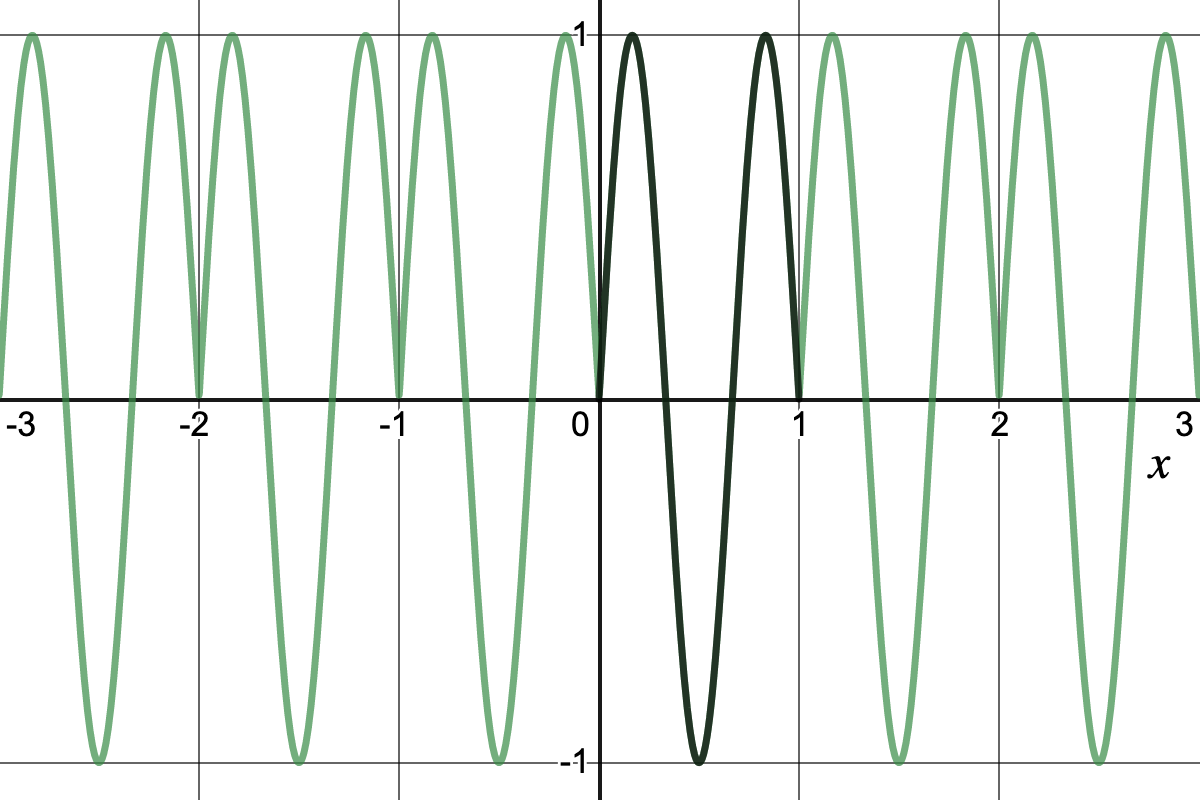
\includegraphics[width=\textwidth]{Figures/sin3pi-series2.png}
					\caption{Approximating $\sin\left(\frac{3\pi x}{L}\right)$ in black.}
				\end{subfigure}
				~ 
				\begin{subfigure}[h]{0.4\textwidth}
					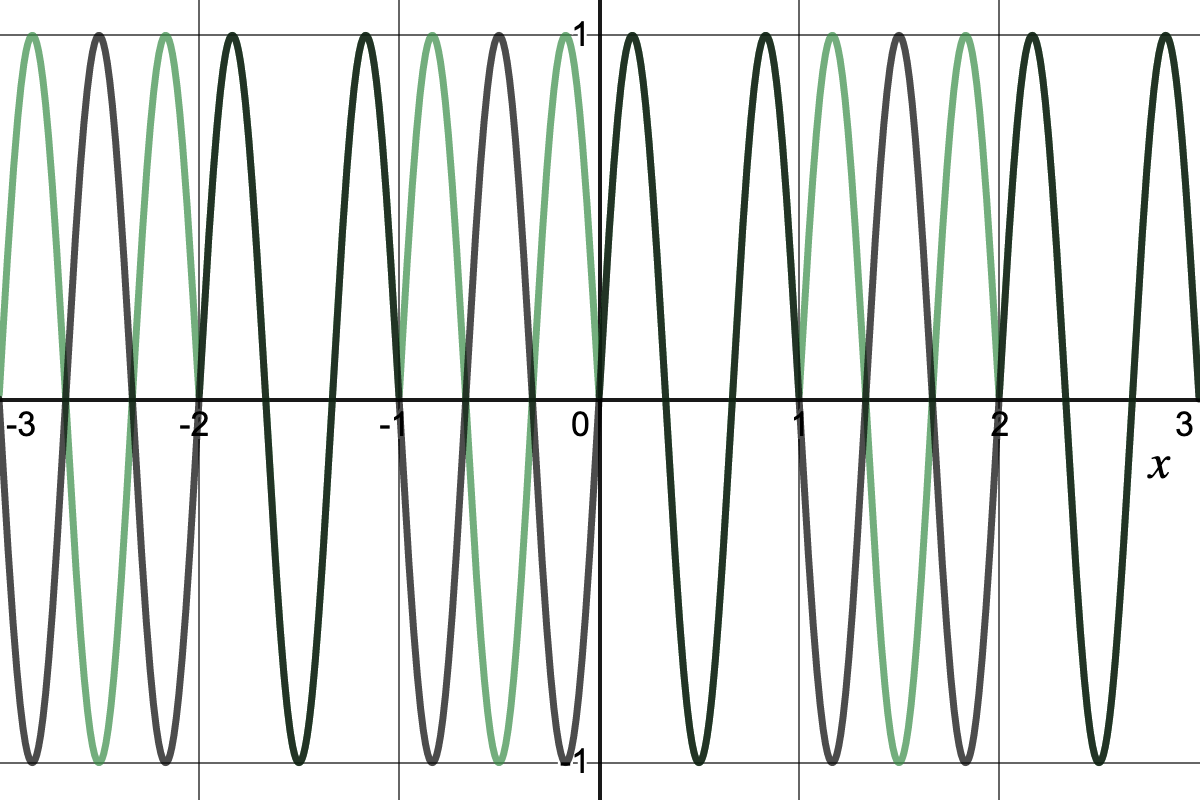
\includegraphics[width=\textwidth]{Figures/sin3pi-series1.png}
					\caption{Approximating $\sin\left(\frac{3\pi x}{L}\right)$ in black.}
				\end{subfigure}
			\end{figure}
		
			\item First, we compute
				\[
				a_0 = \innprod{\delta(x-L/2)}{1} = \frac{1}{L} \int_0^L \delta(x-L/2) dx = \frac{1}{L}.
				\]
				Then, we have
				\begin{align*}
				a_n &= \innprod{\delta(x-L/2)}{\sqrt{2}\cos\left(\frac{2n\pi x}{L}\right)}\\
				& = \frac{1}{L} \int_0^L \delta(x-L/2) \sqrt{2}\cos\left(\frac{2n \pi x}{L}\right)dx\\
				&= \sqrt{2}{L} \cos(n\pi)\\
				&= (-1)^n \frac{\sqrt{2}}{L}.
				\end{align*}
				Finally, we compute
				\begin{align*}
					b_n &= \innprod{\delta(x-L/2)}{\sqrt{2}\sin\left(\frac{2n\pi x}{L}\right)}\\
					&= \frac{1}{L} \int_0^L \delta(x-L/2)\sqrt{2}\sin\left(\frac{2n \pi x}{L}\right)dx\\
					&= \frac{\sqrt{2}}{L} \sin(n\pi)\\
					&= 0.
				\end{align*}
				Hence, our Fourier series is given by
				\[
				\boxed{\delta(x-L/2)) = \frac{1}{L} + \sum_{n=1}^\infty (-1)^n \frac{2}{L} \cos\left(\frac{2n\pi x}{L}\right).}
				\]
					\begin{figure}[H]
								\centering
								\begin{subfigure}[h]{0.4\textwidth}
									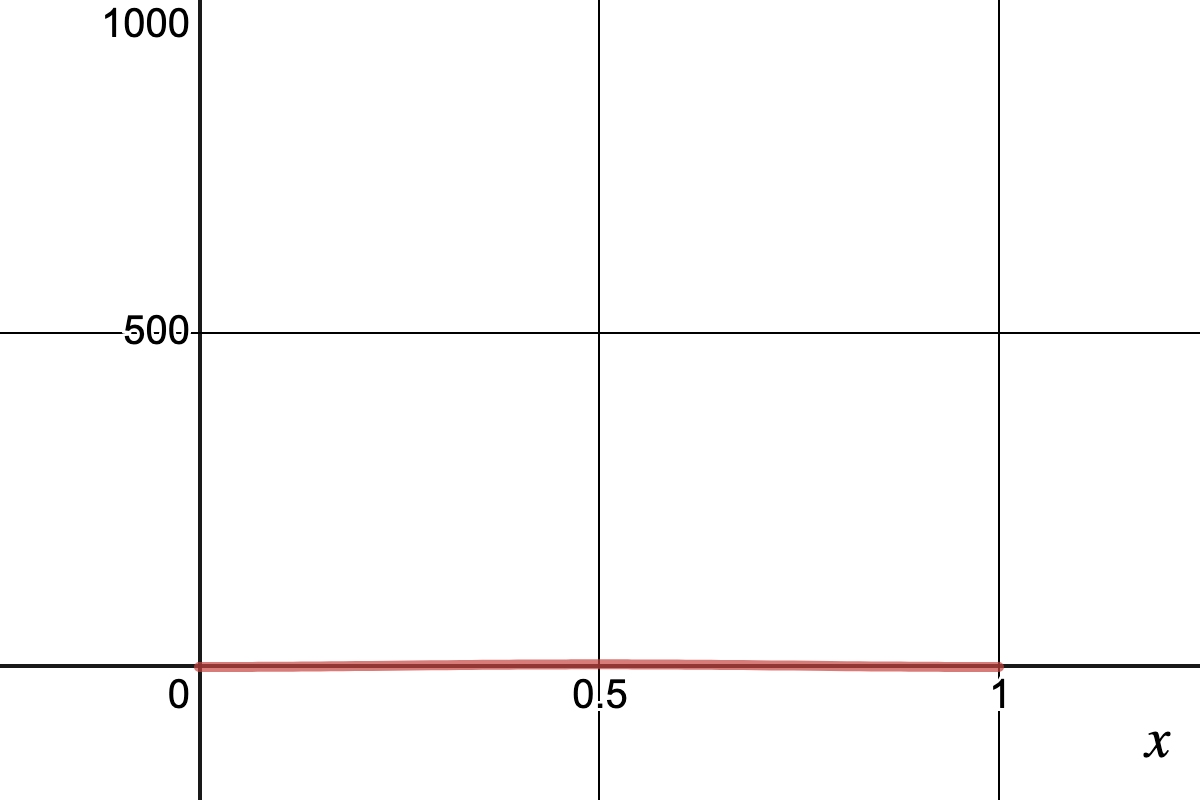
\includegraphics[width=\textwidth]{Figures/delta_N=1.png}
									\caption{$N=1$ approximation to $\delta(x-L/2)$.}
								\end{subfigure}
								~ 
								\begin{subfigure}[h]{0.4\textwidth}
									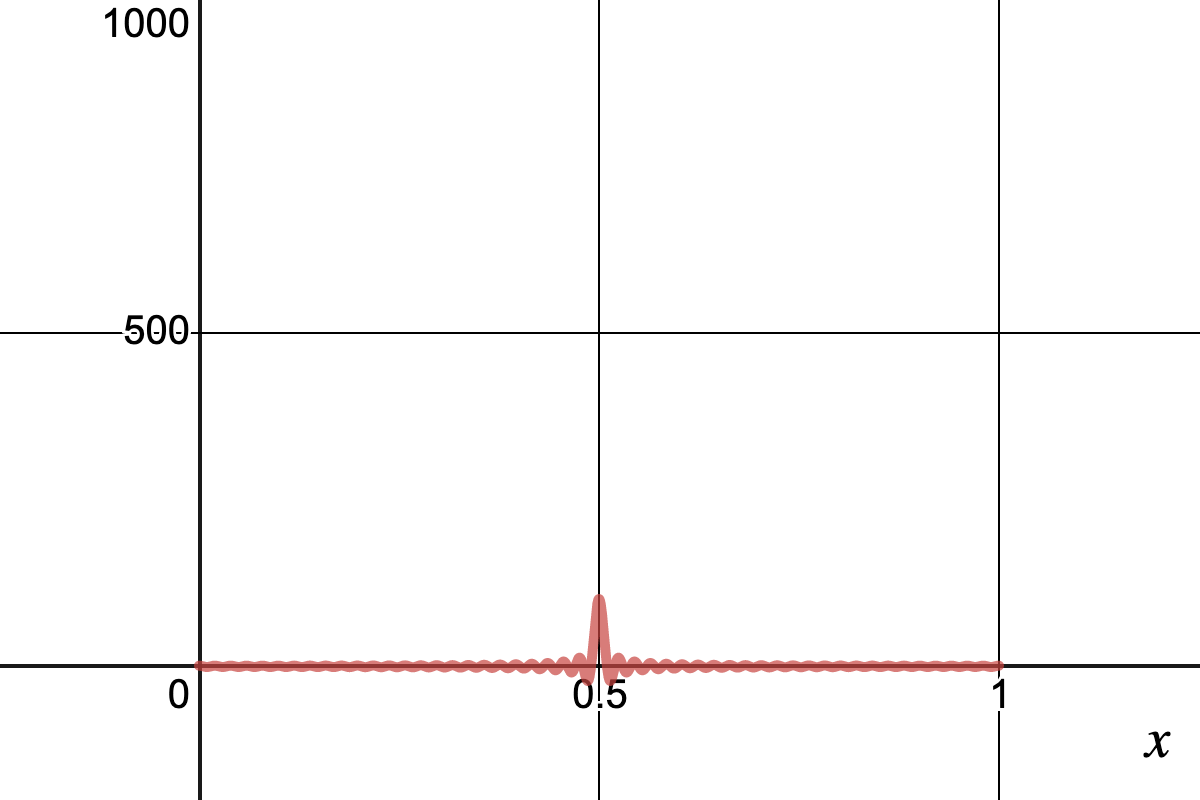
\includegraphics[width=\textwidth]{Figures/delta_N=50.png}
									\caption{$N=50$ approximation to $\delta(x-L/2)$.}
								\end{subfigure}\\
								
								\begin{subfigure}[h]{0.4\textwidth}
									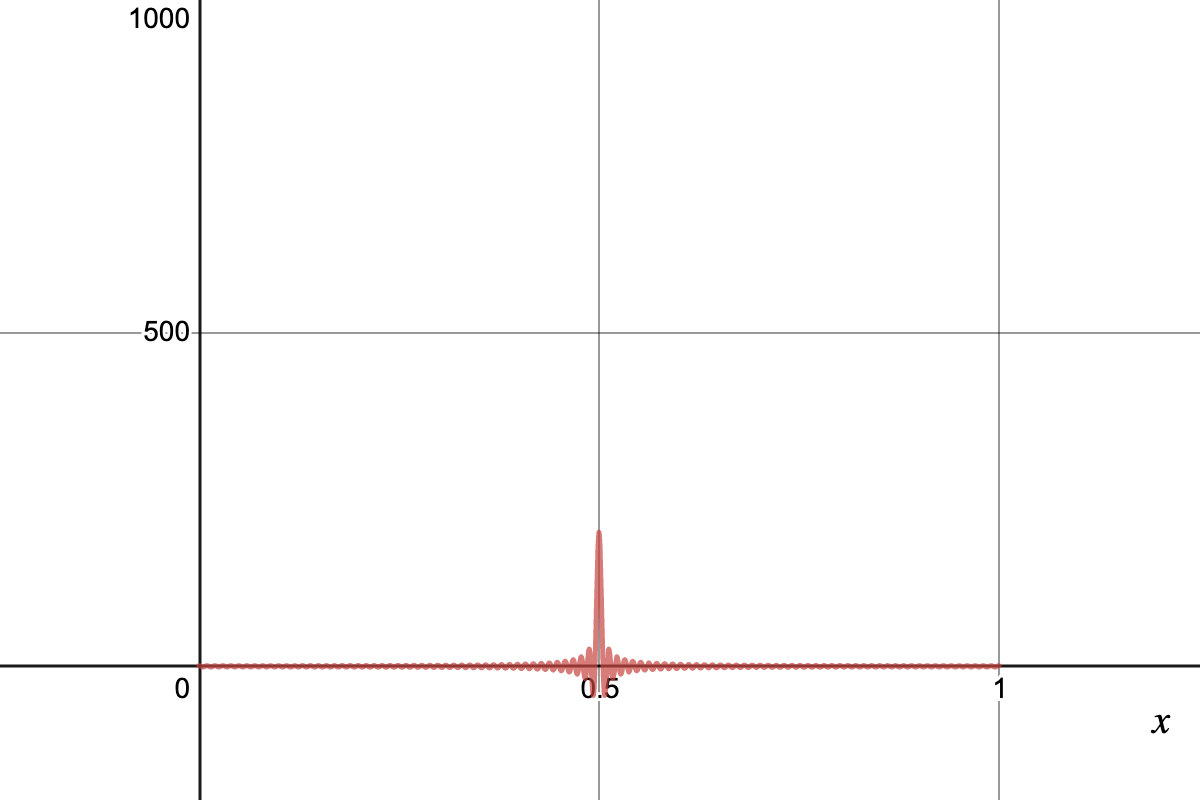
\includegraphics[width=\textwidth]{Figures/delta_N=100.png}
									\caption{$N=100$ approximation to $\delta(x-L/2)$.}
								\end{subfigure}			
								~
								\begin{subfigure}[h]{0.4\textwidth}
									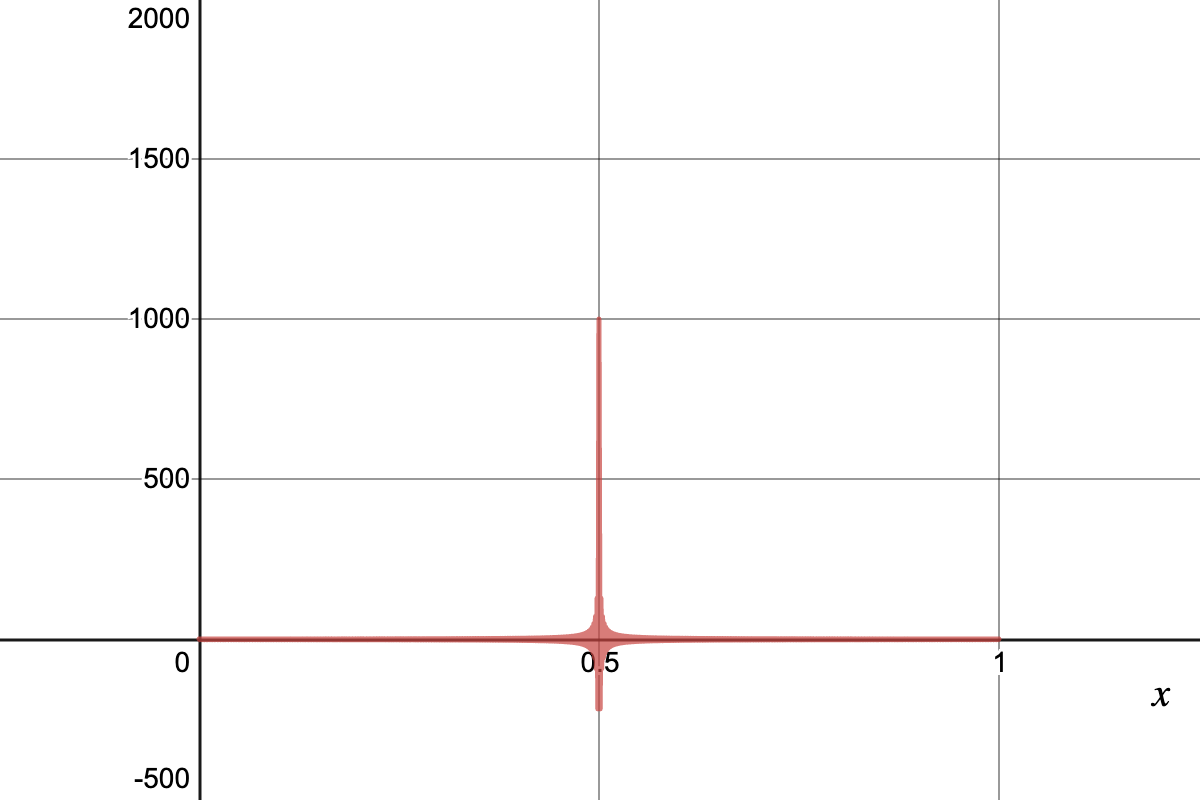
\includegraphics[width=\textwidth]{Figures/delta_N=500.png}
									\caption{$N=500$ approximation to $\delta(x-L/2)$.}
								\end{subfigure}													
							\end{figure}
		\end{enumerate}
	
\end{solution}

\newpage
\begin{problem}
Consider a function $f(x)$ that describes the height of a rubber string with rest length $L$. We can attach the ends of the string at $x=0$ and $x=L$ by requiring that $f(0)=f(L)=0$.  Then, one can subject the string to an external force $g(x)$ and find the profile of the string by solving
\[
-\frac{d^2}{dx^2} f(x) = g(x).
\]
\begin{enumerate}[(a)]
	\item Let $g(x)=\delta(x-L/2)$ and let $f(x)$ be given by some Fourier series.  Using the equation above, solve for the coefficients of the Fourier series for $f(x)$.
	\item Plot the Fourier series for $f(x)$ for $N=1,5,50$.
\end{enumerate}
This is an extremely important to solve. The fact that we can determine a solution $f(x)$ where the external force is the Dirac delta function means that we have the ability to determine a the deformation of a string from a point force.
\end{problem}
\begin{solution}~
	\begin{enumerate}[(a)]
		\item	Here we let $f(x)$ be written as an arbitrary Fourier series by
		\[
			f(x) = a_0 + \sum_{n=1}^\infty a_n \sqrt{2} \cos\left(\frac{2n \pi x}{L}\right) + \sum_{n=1}^\infty b_n \sqrt{2}\sin\left(\frac{2n\pi x}{L}\right).
		\]
		Then we can put
		\[
		-\frac{d^2}{dx^2} f(x) = \frac{4n^2\pi^2}{L^2} \left(\sum_{n=1}^\infty a_n \sqrt{2} \cos\left(\frac{2n \pi x}{L}\right) + \sum_{n=1}^\infty b_n \sqrt{2}\sin\left(\frac{2n\pi x}{L}\right)\right).
		\]
		Setting the left hand side of the ODE equal to the right, we have
		\begin{align*}
			-\frac{d^2}{dx^2}f(x) &= g(x)\\
			\frac{4n^2\pi^2}{L^2} \left(\sum_{n=1}^\infty a_n \sqrt{2} \cos\left(\frac{2n \pi x}{L}\right) + \sum_{n=1}^\infty b_n \sqrt{2}\sin\left(\frac{2n\pi x}{L}\right)\right) &= \frac{1}{L} + \sum_{n=1}^\infty (-1)^n \frac{2}{L} \cos\left(\frac{2n\pi x}{L}\right).
		\end{align*}
		Hence, we just need to determine the coefficients $a_0$, $a_n$, and $b_n$ for our function $f(x)$. It's clear to see that the $b_n$ terms for $f(x)$ must be zero. Solving for the $a_n$ terms, we find
		\[
		\frac{4n^2\pi^2}{L^2} a_n= (-1)^n \frac{2}{\sqrt{2}L},
		\]
		which yields
		\[
		a_n = (-1)^n \frac{L}{2\sqrt{2}n^2\pi^2}.
		\]
		At this point, we have that
		\[
		f(x) = a_0 + \sum_{n=1}^\infty (-1)^n \frac{L}{2n^2\pi^2}\cos\left(\frac{2n\pi x}{L}\right).
		\]
		We can determine $a_0$ by inforcing our boundary conditions. Namely, we take
		\begin{align*}
		0=f(0)&= a_0 + \sum_{n=1}^\infty (-1)^n \frac{L}{2n^2\pi^2}\\
		&=a_0 -\frac{L}{24},
		\end{align*}
		where I used WolframAlpha to evaluate the infinite series above.  This means that $a_0 = \frac{L}{24}$. Thus, we arrive at
		\[
		\boxed{f(x) = \frac{L}{24} + \sum_{n=1}^\infty (-1)^n \frac{L}{2n^2\pi^2}\cos\left(\frac{2n\pi x}{L}\right).}
		\]
		
							\begin{figure}[H]
										\centering
										\begin{subfigure}[h]{0.3\textwidth}
											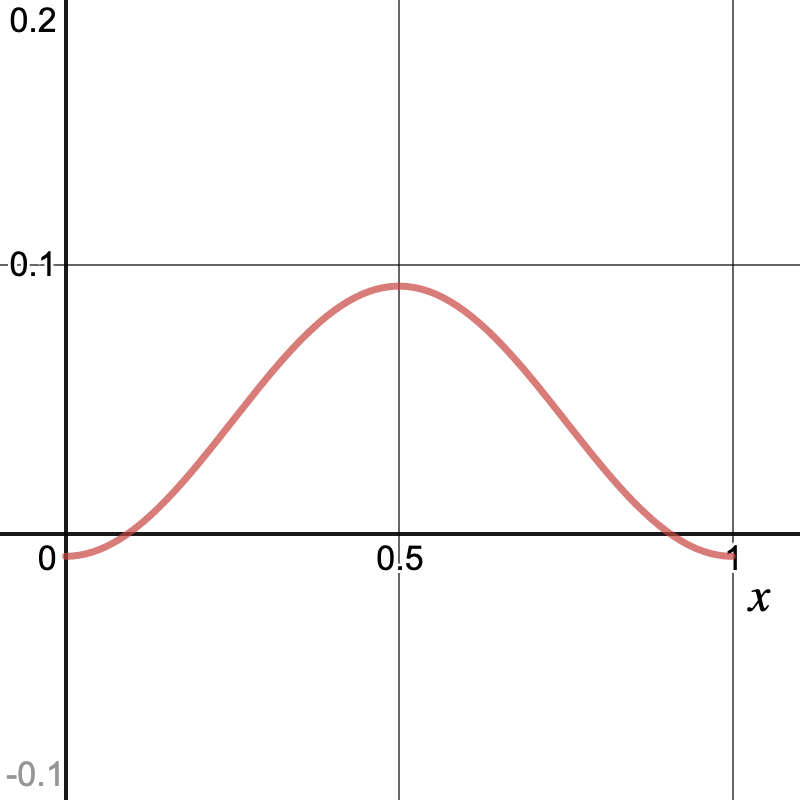
\includegraphics[width=\textwidth]{Figures/fund_soln_N=1.png}
											\caption{$N=1$ approximation to the differential equation..}
										\end{subfigure}
										~ 
										\begin{subfigure}[h]{0.3\textwidth}
											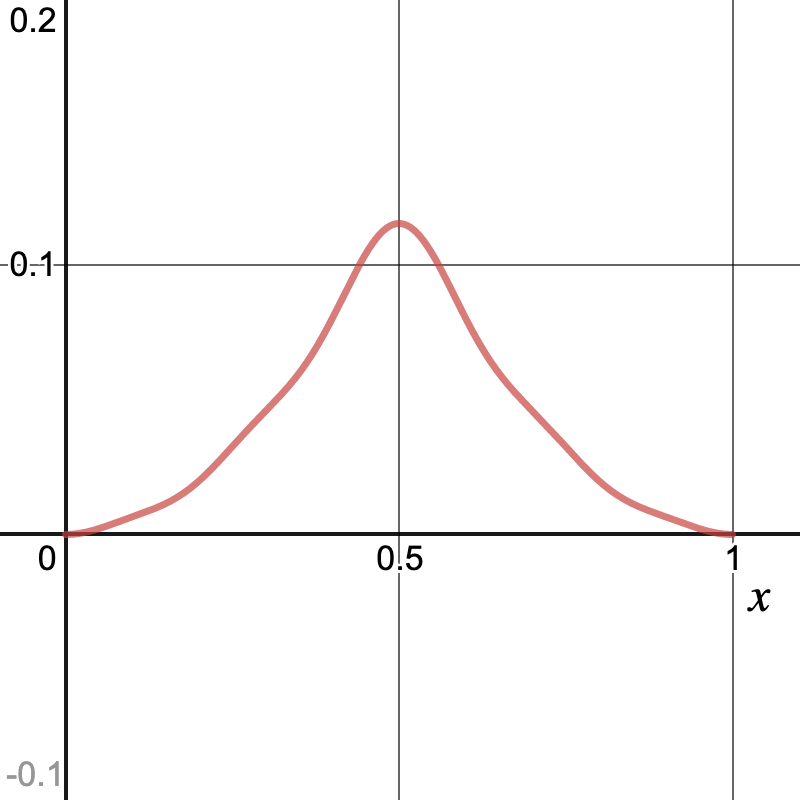
\includegraphics[width=\textwidth]{Figures/fund_soln_N=5.png}
											\caption{$N=5$ approximation to the differential equation..}
										\end{subfigure}
										~
										\begin{subfigure}[h]{0.3\textwidth}
											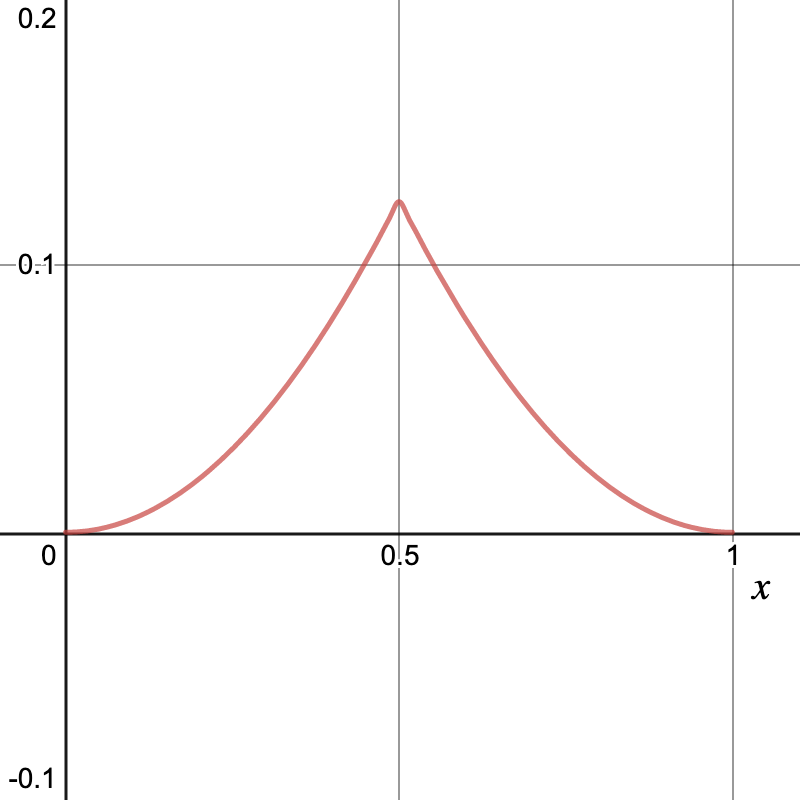
\includegraphics[width=\textwidth]{Figures/fund_soln_N=50.png}
											\caption{$N=50$ approximation to the differential equation..}
										\end{subfigure}														
									\end{figure}
	\end{enumerate}
\end{solution}


\newpage
\begin{problem}
Compute the following Fourier transforms (using a table or WolframAlpha if need be).  
\begin{enumerate}[(a)]
	\item $\sin(3\pi x)$.
	\item $e^{\frac{-x^2}{2}}$.
	\item $\delta(x)$.
\end{enumerate}
\end{problem}
\begin{solution}~
	\begin{enumerate}[(a)]
		\item To compute the Fourier transform, one could use a table. However, we can take
		\[
		\fourier{\sin(3\pi x)} = \int_{-\infty}^\infty \sin(3\pi x)e^{-i2\pi kx}dx.
		\]
		The techniques used to compute this integral by hand are found in complex analysis. Specifically, one uses the fact that $\sin(3\pi x)$ is an analytic function on $\C$ as well as the method of contour integration (seen here: \url{https://en.wikipedia.org/wiki/Contour_integration}). This is not a topic for our class (though we will learn how to integrate along curves).
		
		Anyways, computing this Fourier transform yields
		\[
		\boxed{\fourier{\sin(3\pi x)} = \frac{\delta\left(k-\frac{3}{2}\right)-\delta\left(k+\frac{3}{2}\right)}{2i}.}
		\] 
		Here, I used a table to compute this (as WolframAlpha claims the integral does not converge).
		\item Again, we want to compute
		\[
		\fourier{e^{\frac{-x^2}{2}}} = \int_{-\infty}^\infty e^{\frac{-x^2}{2}}e^{-i2\pi kx}dx.
		\]
		I was able to compute this using WolframAlpha by entering
		\begin{verbatim}
			integrate[e^(-x^2/2)e^{-i2*pi*k*x},{x,-infty,infty}]
		\end{verbatim}
		This yields
		\[
		\boxed{\fourier{e^{\frac{-x^2}{2}}} = \sqrt{2\pi}e^{-2\pi^2k^2}.}
		\]
		One thing to note here is that the Fourier transform of a Gaussian is a Gaussian!
		\item Since, in some sense, the Dirac delta is a Gaussian function (with a variance of zero), we expect to get another type of Gaussian out as well. Let's see what happens. We take
		\begin{align*}
			\boxed{\fourier{\delta(x)} = \int_{-\infty}^\infty \delta(x) e^{-i2\pi k x}dx = 1.}
		\end{align*}
		The constant 1 function is much like a Gaussian with an infinite variance! This is maybe a ``handwavy" way to look at this.
		\end{enumerate}
\end{solution}

\newpage
\begin{problem}
A common application for the Fourier transform is to solve differential equations whose domain is time $t\in [0,\infty)$. We can model how a point $x$ on a rubber string oscillates over time consider the differential equation
\[
u''(t)+v^2u(t)=0,
\]
with initial conditions $u(0)=L$ and $u'(0)=0$. Here $u(t)$ is the displacement of the string at position $x$ with the initial conditions describing the string being pulled tight at time $t=0$.
\begin{figure}[H]
	\centering
	\def\svgwidth{\columnwidth}
	\input{point_on_string.pdf_tex}
\end{figure}
To solve this equation, we could use use methods we learned previously, or apply the Fourier transform to the whole equation by
\[
\fourier{u''(t)+v^2u(t)}=\fourier{0}.
\]
\begin{enumerate}[(a)]
	\item Compute the Fourier transform above.
	\item One should then have a new equation
	\[
	-4\pi^2k^2\hat{u}(k)+v^2\hat{u}(k)=0.
	\]
	Solve this new equation for $k$.
	\item One should have two values $k_1$ and $k_2$ from the work in (b).  This corresponds to the solution
	\[
	\hat{u}(k)=\delta(k-k_1) \qquad \textrm{and} \qquad \hat{u}(k)=\delta(k-k_2).
	\]
	Compute the inverse Fourier transform of the two delta functions. A linear combination of these correspond to your solution $u(t)$.
\end{enumerate}
\end{problem}
\begin{solution}~
	\begin{enumerate}[(a)]
		\item We have that the Fourier transformed equation is given by
		\[
		-4\pi^2k^2 \hat{u}(k)+v^2 \hat{u}(k) = 0,
		\]
		since the Fourier transform converts differentiation into multiplication.  
		\item Indeed, we have this equation.  If we solve this equation for $k$, we have
		\[
		(-4\pi^2k^2+v^2)\hat{u}(k)=0,
		\]
		which yields
		\[
		k = \pm \frac{|v|}{2\pi}.
		\]
		\item Put $k_1 = -\frac{|v|}{2\pi}$ and $k_2=\frac{|v|}{2\pi}$.  Thus, we get
		\[
		\hat{u}(k) = \delta\left(k+\frac{|v|}{2\pi}\right) \qquad \textrm{and} \qquad \hat{u}(k) = \delta\left(k-\frac{|v|}{2\pi}\right).
		\]
		Then we have that
		\[
		\fourier{\delta\left(k+\frac{|v|}{2\pi}\right)} = e^{-ivt}
		\]
		and
		\[
		\fourier{\delta\left(k-\frac{|v|}{2\pi}\right)} = e^{ivt}.
		\]
		If we take a linear combination of these solutions we arrive at
		\[
		u(t) = C_1 e^{ivt}+C_2 e^{-ivt},
		\]
		which is the solution we have found for the harmonic oscillator equation before!
	\end{enumerate}
\end{solution}




\end{document}